\reviewer
% Comment 1
\begin{revcomment}
  The authors should explain the most important achievements of the proposed method quantitatively, in the abstract.
\end{revcomment}
\begin{revresponse}

Thanks for the reviewer's valuable feedback. We have carefully considered this suggestion and made the following modifications to address the reviewer's concern:


By introducing the shortest path (SP) of the battery, the greedy algorithm transforms the enumeration of switch states in the brute force algorithm into the combination of the SPs, resulting in more efficient computation of the maximum allowable current (MAC).
We have also provided a theoretical estimation of the improvement, which is proportional to $2^{N_s - N_b} N_s \log_{10} N_b$ for an RBS with $N_b$ batteries and $N_s$ switches.


Here is the specific content we added in the abstract:
\begin{changes}
  \ExecuteMetaData[2-main]{reviewer1-comment1}
\end{changes}


We hope the above content provide a more quantitative explanation of the achievements of our proposed method in the abstract. 

\end{revresponse}

% Comment 2
\begin{revcomment}
  The literature review in the introduction section is very short, and the related works, especially the works published in recent years, have not been well reviewed and compared, and the conclusions about the existing research gaps have not been presented.
\end{revcomment}
\begin{revresponse}

Considering the Reviewer's suggestion, we have expanded the literature review in the introduction section to provide a comprehensive overview of the existing RBS structures (cited as \cite{ci2007novel,9209774,engelhardt2021double,visairoReconfigurableBatteryPack2008,lawsonSoftwareConfigurableBattery2012,he2014reconfiguration,kim2009dynamic} in revised manuscript) and related works on structure analyses (cited as \cite{han2021analysis,chenSneakCircuitTheory2021} in revised manuscript). 
Although many RBS structures have been proposed for different purposes, such as dynamically adjusting the output voltage , increasing energy utilization efficiency, and improving the system's ability to recover from battery failures, these structures also bring challenges in design and control of the systems.
Therefore, several works on structure analyses, like the maximum switch current and the short-circuit problem, have been proposed to tackle these challenges recently.
However, determining the MAC of RBSs remains blank accroding to our literature review.
A straightforward method is to enumerate all possible switch states.
But this method has exponentially increasing computational complexity with the number of switches, and is too ineffection to apply.


Here is the specific modification we made in the introduction:
\begin{changes}
  \ExecuteMetaData[2-main]{reviewer1-comment2}
\end{changes}

  
Thanks again for the reviewer's comments, which have greatly improved the quality and comprehensiveness of our manuscript. 
  
\end{revresponse}

% Comment 3
\begin{revcomment}
  It is necessary for the authors to clearly state research contribution and achievements as bullet points at the end of the Introduction section.
\end{revcomment}
\begin{revresponse}

We appreciate and accept your suggestion and have added a clear statement of the contributions in the second-to-last paragraph of the Introduction, as shown below:
\begin{changes}
  \ExecuteMetaData[2-main]{reviewer1-comment3}
\end{changes}


\end{revresponse}

% Comment 4
\begin{revcomment}
  The authors need to present the complexity of their proposed method and compare it with some other state-of-the-art or successful classic methods.
\end{revcomment}
\begin{revresponse}

We totally agree with the reviewer's suggestion.
It is indeed necessary to analyze the complexity of the proposed method and compare it with other existing methods.


We have derived the average time complexity of our proposed greedy algorithm-based MAC determination method to be approximately $O(2^{N_b}N_s^2\log_{10} N_b)$, where $N_b$ and $N_s$ are the number of batteries and switches, respectively.
However, as mentioned in our response to Comment 2, there is a blank in the literature regarding MAC determination methods.
The brute force method, the most straightforward and intuitive method, is used as a benchmark for comparison, the time complexity of which is $O(2^{N_s}N_s^3)$.
Since the number of switches in RBS is typically 3 to 5 times the batteries, the method we proposed is theoretically more efficient than the brute force method.
It has been validated by the case study in the manuscript.


The detailed derivation and discussion of the above points have been added to the revised manuscript under the Discussion subsection.
Here is the specific content:
\begin{changes}
  \ExecuteMetaData[2-main]{reviewer1-comment4}
\end{changes}

\end{revresponse}

% Comment 5
\begin{revcomment}
  The authors don't discuss the limitations of the study correctly.
\end{revcomment}
\begin{revresponse}

We are sorry for our negligence of the limitations of the study. 
As far as we are concerned, although the method we proposed is strongly efficient than the brute force method, it still has a exponential relationship with the number of batteries.
That means unsufferable time will be costed for systems with large number of batteries.


Here is the specific content we added in the discussion:
\begin{changes}
  \ExecuteMetaData[2-main]{reviewer1-comment5}
\end{changes}

\end{revresponse}


% Comment 6
\begin{revcomment}
  Some typos should be double check.
\end{revcomment}
\begin{revresponse}

We are very sorry for our incorrect writing, and have carefully checked the manuscript and corrected the typos. 
  
\end{revresponse}

% Comment 7
\begin{revcomment}
  The author should explain more why solution quality of their proposed approach is much better than the others?
\end{revcomment}
\begin{revresponse}

We appreciate the reviewer's concern regarding the explanation of why the solution quality of our proposed approach is better to others. 
However, after careful literature research, we would like to clarify that there are currently no existing works on the MAC determination of RBSs that we could compare our solution with. 
Therefore, it is not possible to directly compare the solution quality of our proposed approach with others.
  
\end{revresponse}

% Comment 8
\begin{revcomment}
  Authors should mention some novel works in the field in the introduction, specially refer to this 2023 reference: An efficient lightweight algorithm for scheduling tasks onto dynamically reconfigurable hardware using graph-oriented simulated annealing, which uses graph-based method. Mention and refer to it in the introduction section.
\end{revcomment}
\begin{revresponse}

Thanks to the reviewer's suggestion, we have introduced two novel works in the RBS structure analysis field in the introduction, which respectively study the maximum switch current and the short-circuit problem.
Here is the specific content we added in the introduction:
\begin{changes}
  \ExecuteMetaData[2-main]{reviewer1-comment8}
\end{changes}


The reviewer also mentioned the work \enquote{An efficient lightweight algorithm for scheduling tasks onto dynamically reconfigurable hardware using graph-oriented simulated annealing}, sepcially.
After carefully reading and fully discussion, we reached a conclusion that this paper is not relevant to our research.
Although this paper uses a graph-based method, whose name is similar to the method described in our paper, it mainly studies the task scheduling problem in time series.
While our research is about the maximum allowable current of RBS structure, which belongs to the field of structure analysis.
Therefore, we think it is not appropriate to include this paper in our introduction and will not cite it.
  
\end{revresponse}

% Comment 9
\begin{revcomment}
  Authors need to explain about the accuracy, sufficiency and reliability of their results? How do they verify and validate the results?
\end{revcomment}
\begin{revresponse}

Thanks for the reviewer's valuable feedback. 
We have carefully considered the reviewer's question.
In response, we complemented the computation and validation with the brute force method and provided more detailed explanation and discussion.


In the Case study section of the paper, we investigated three RBS structures, two of which are from published literatures (see references \cite{lawsonSoftwareConfigurableBattery2012,visairoReconfigurableBatteryPack2008} in revised manuscript) and the other is designed by ourselves, as shown in Figs. \ref{fig:study-stru-Lawson-comment}, \ref{fig:study-stru-Visairo-comment}, and \ref{fig:study-stru-my-comment}, respectively.
The results of the three RBS structures calculated by our proposed method are shown in Tabs. \ref{tab:study-results-Lawson-greedy}, \ref{tab:study-results-Visairo-greedy}, and \ref{tab:study-results-my-greedy}, respectively.
The results by brute force method are shown in Tabs. \ref{tab:study-results-Lawson-brute}, \ref{tab:study-results-Visairo-brute}, and \ref{tab:study-results-my-brute}, respectively.


On the one hand, as shown in the Tabs. \ref{tab:study-results-Lawson-greedy} -- \ref{tab:study-results-my-brute}, the reconfigured structure results from greedy algorithm are consistent with the results from the brute force algorithm.
Since the brute force algorithm enumerates all possible reconfigured structures, it ensures that we obtain the global optimal solution.
On the other hand, the output current of the system calculated by our directed graph model is consistent with the experience and common sense.
To illustrate this, the RBS in Fig. \ref{fig:study-stru-my-comment} is taken as an example here.
The four batteries in this system can be divided into two groups: gourp $g_A$ has $B_1$ and $B_2$; group $g_B$ has $B_3$ and $B_4$.
The relationship between the two batteries in each group can be switched between series and parallel by reconfigurating the structure.
While the two groups can only connect in series or disconnect.
Therefore, this system's MAC is the maximum of the MAC of the two groups (i.e., $\max[\text{MAC}(g_A),\text{MAC}(g_B)]$).
Both $g_A$ and $g_B$ are the two-battery and degenerated structure of the RBS in Fig. \ref{fig:study-stru-Visairo-comment}, and have the same MAC (i.e., 2).
Therefore, the MAC of the RBS in Fig. \ref{fig:study-stru-my-comment} is 2, consistent with the result shown in Tab. \ref{tab:study-results-my-greedy}.


We hope the above content can address the reviewer's concerns.
The above content corresponds to lines 276 to 283, and lines 289 to 294 of our revised manuscript without changes marked.

\begin{figure}[htbp]
    \centering
    \begin{subfigure}[b]{0.2\textwidth}
        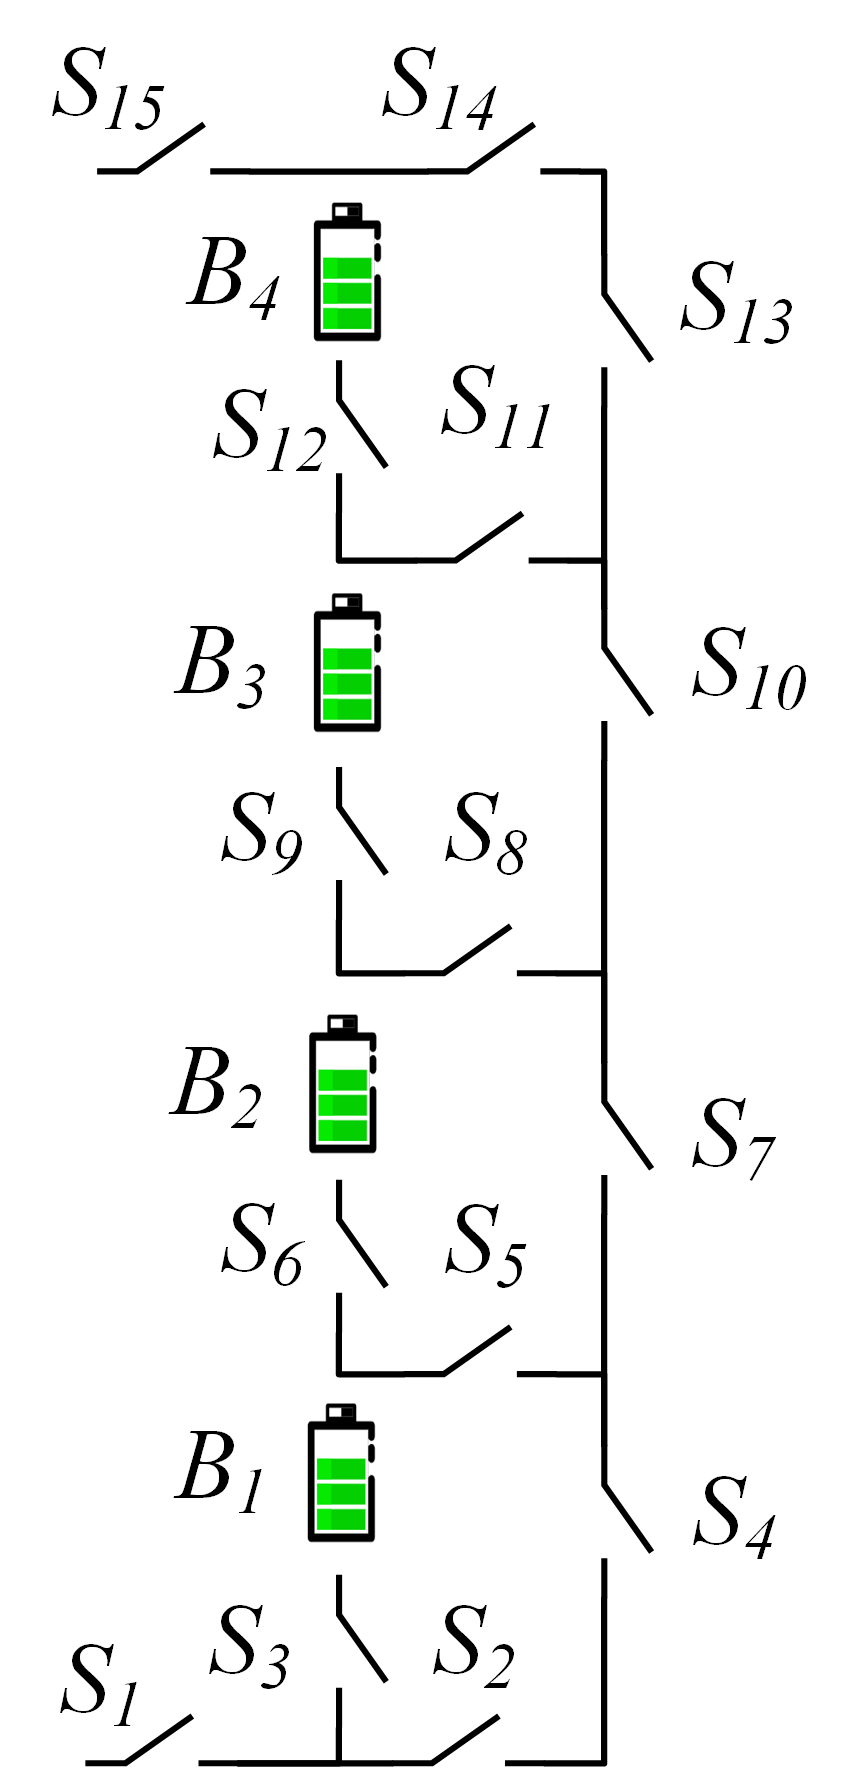
\includegraphics[width=\textwidth]{stru-L-origin.png}
        \caption{}
        \label{fig:study-stru-Lawson-comment}
    \end{subfigure}
    \hspace{0.02\textwidth}
    \begin{subfigure}[b]{0.4\textwidth}
        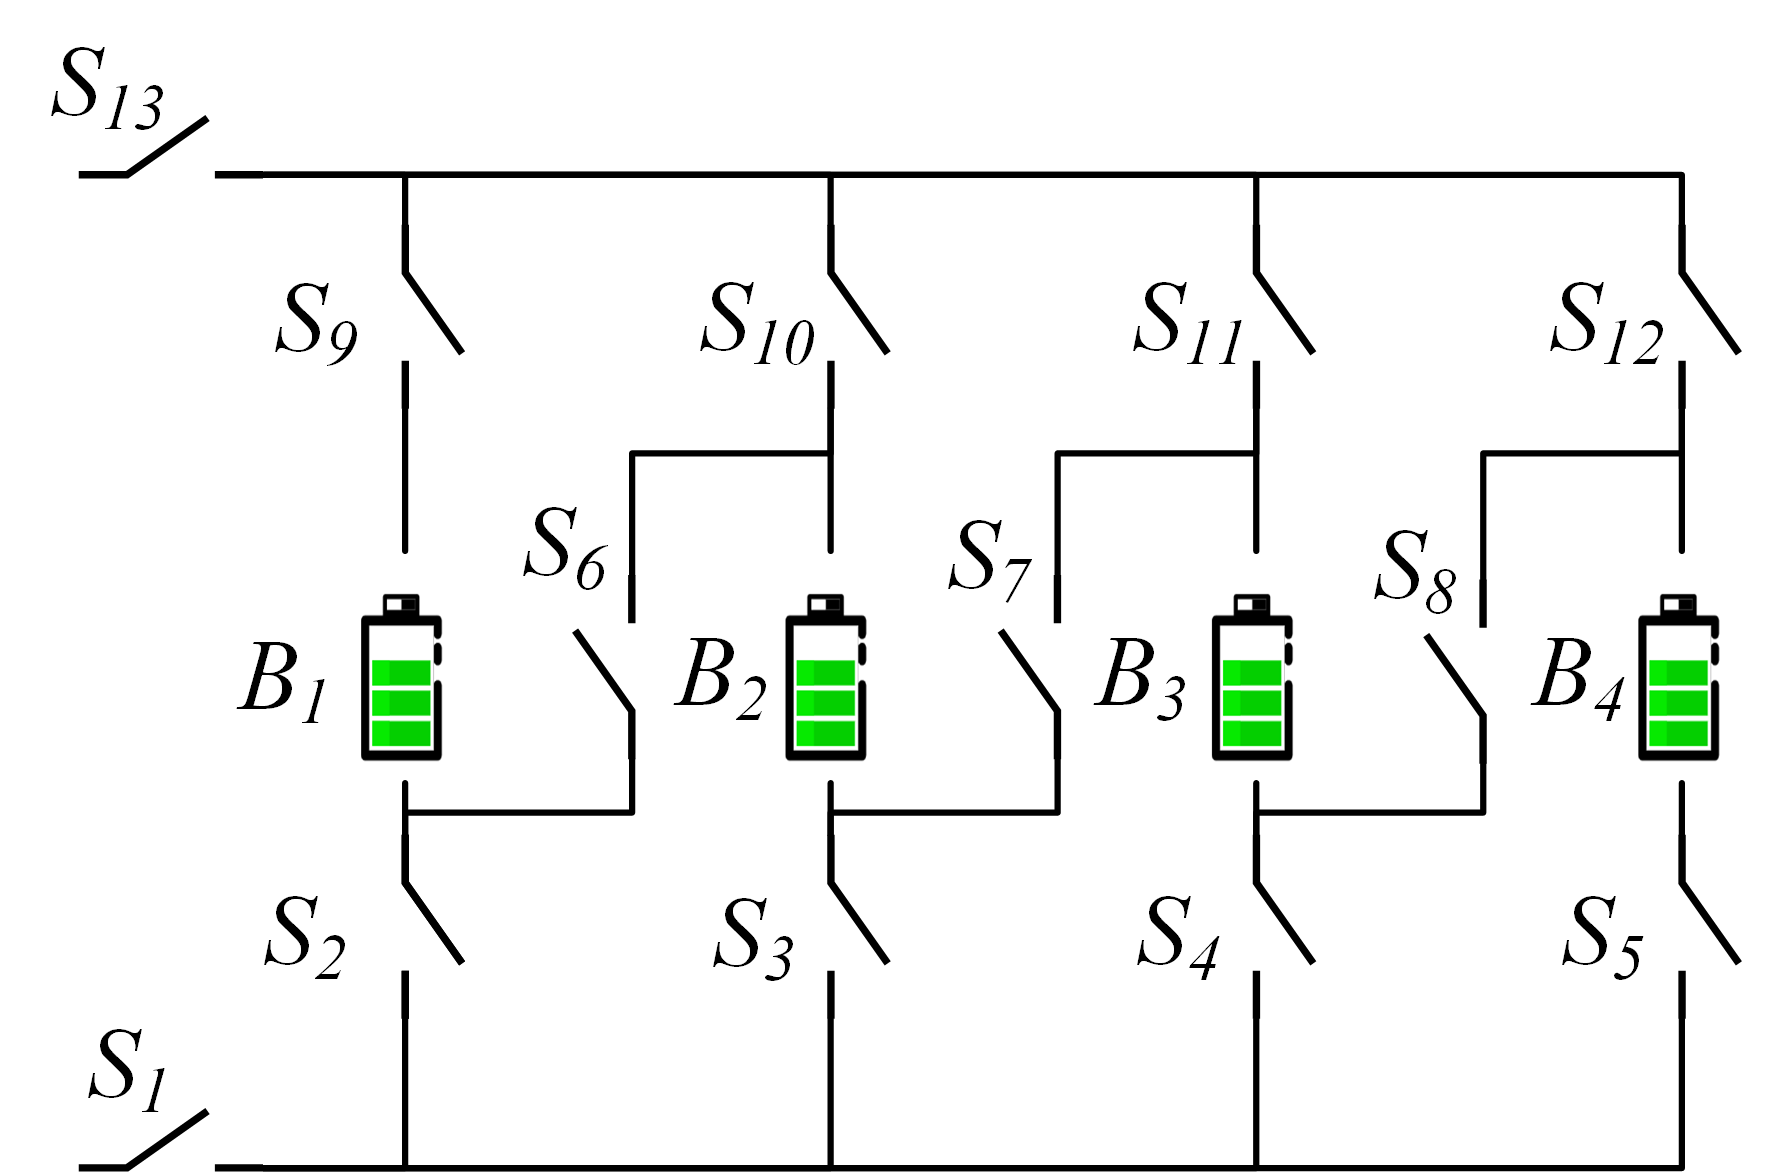
\includegraphics[width=\textwidth]{stru-V-origin.png}
        \caption{}
        \label{fig:study-stru-Visairo-comment}
    \end{subfigure}
    \hspace{0.02\textwidth}
    \begin{subfigure}[b]{0.31\textwidth}
        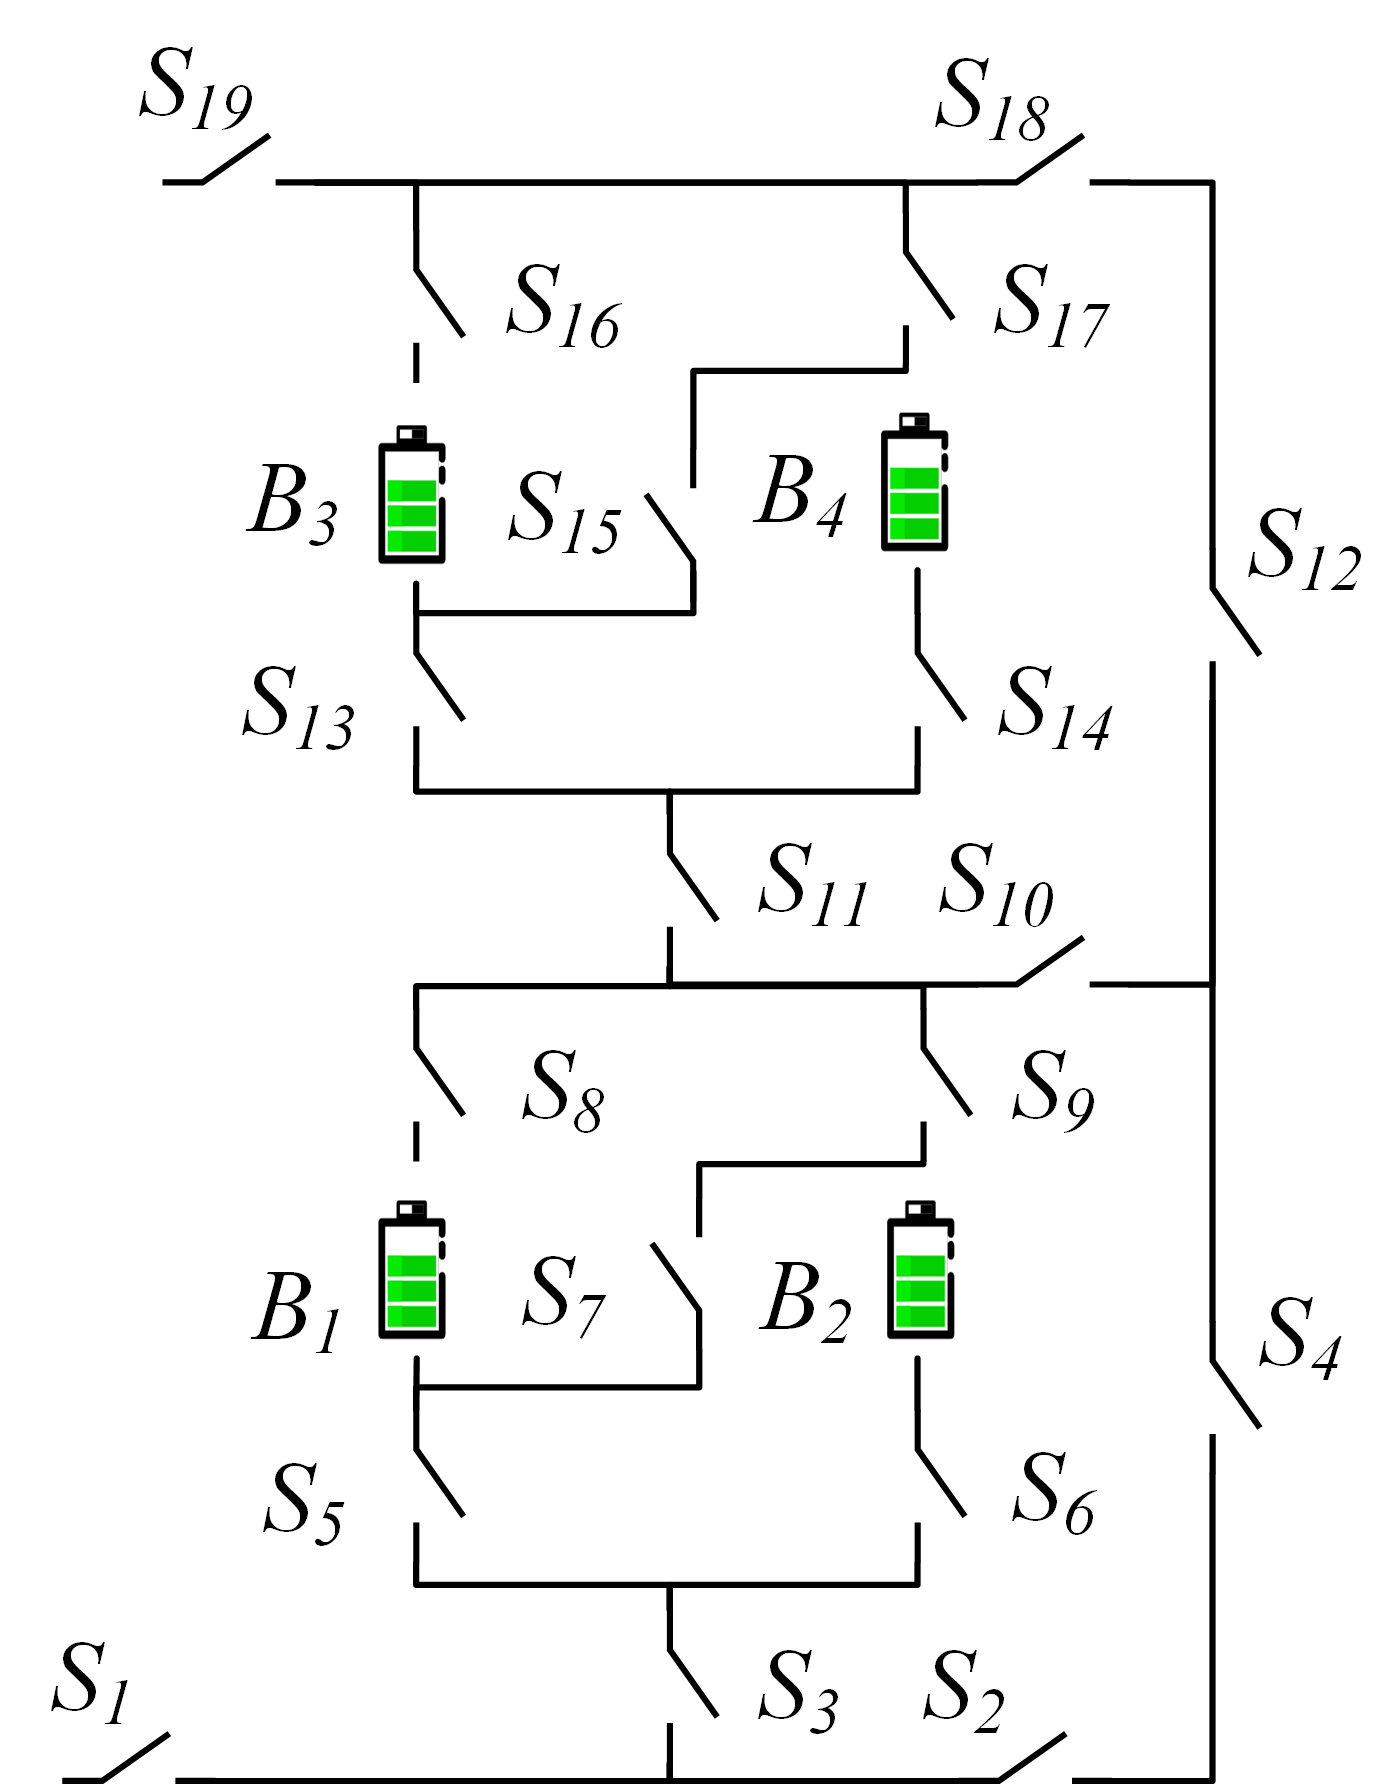
\includegraphics[width=\textwidth]{stru-my-origin.png}
        \caption{}
        \label{fig:study-stru-my-comment}
    \end{subfigure}
    \caption{The four-battery RBS structures proposed by (a)Lawson\cite{lawsonSoftwareConfigurableBattery2012}, (b)Visairo\cite{visairoReconfigurableBatteryPack2008} and (c)this paper.}
\end{figure}

\begin{table}[htbp]
  \centering
    \caption{MAC Calculating result of the RBS structure in Figure \ref{fig:study-stru-Lawson-comment} with our method.}
    \begin{tabular}{cc}
    \toprule
        Structure & Figure \ref{fig:study-stru-Lawson-comment} with 4 batteries and 15 switches  \\
    \midrule
    Switch ON & $S_1$,$S_3$,$S_5$,$S_7$,$S_{10}$,$S_{13}$,$S_{14}$,$S_{15}$ \\
    $I_o$ & $u_b/(R_o+r_b)$ \\
    $\bm{I}_b$ & $[u_b/(R_o+r_b),0,0,0]$ \\
    $\max  \eta$     & 1 \\
    computed structure count & 11 \\
    \bottomrule
    \end{tabular}
  \label{tab:study-results-Lawson-greedy}
\end{table}

\begin{table}[htbp]
  \centering
    \caption{MAC Calculating result of the RBS structure in Figure \ref{fig:study-stru-Visairo-comment} with our method.}
    \begin{tabular}{cc}
    \toprule
        Structure & Figure \ref{fig:study-stru-Visairo-comment} with 4 batteries and 13 switches  \\
    \midrule
    Switch ON & $S_1$,$S_2$,$S_3$,$S_4$,$S_5$,$S_9$,$S_{10}$,$S_{11}$,$S_{12}$,$S_{13}$ \\
    $I_o$ & $4u_b/(4R_o+r_b)$ \\
    $\bm{I}_b$ & $[u_b/(4R_o+r_b),u_b/(4R_o+r_b),u_b/(4R_o+r_b),u_b/(4R_o+r_b)]$ \\
    $\max \eta$     & 4 \\
    computed structure count & 1 \\
    \bottomrule
    \end{tabular}
  \label{tab:study-results-Visairo-greedy}
\end{table}

\begin{table}[htbp]
  \centering
    \caption{MAC Calculating result of the RBS structure in Figure \ref{fig:study-stru-my-comment} with our method.}
    \begin{tabular}{cc}
    \toprule
        Structure & Figure \ref{fig:study-stru-my-comment} with 4 batteries and 19 switches  \\
    \midrule
    Switch ON & $S_1$,$S_3$,$S_5$,$S_6$,$S_8$,$S_9$,$S_{10}$,$S_{12}$,$S_{18}$,$S_{19}$ \\
    $I_o$ & $2u_b/(2R_o+r_b)$ \\
    $\bm{I}_b$ & $[u_b/(2R_o+r_b),u_b/(2R_o+r_b),0,0]$ \\
    $\max  \eta$     & 2 \\
    computed structure count & 11 \\
    \bottomrule
    \end{tabular}
  \label{tab:study-results-my-greedy}
\end{table}

\begin{table}[htbp]
  \centering
    \caption{MAC Calculating result of the RBS structure in Figure \ref{fig:study-stru-Lawson-comment} with brute force method.}
    \begin{tabular}{cc}
    \toprule
        Structure & Figure \ref{fig:study-stru-Lawson-comment} with 4 batteries and 15 switches  \\
    \midrule
    Switch ON & $S_1$,$S_3$,$S_5$,$S_7$,$S_{10}$,$S_{13}$,$S_{14}$,$S_{15}$ \\
    $I_o$ & $u_b/(R_o+r_b)$ \\
    $\bm{I}_b$ & $[u_b/(R_o+r_b),0,0,0]$ \\
    $\max \eta$     & 1 \\
    computed structure count & 32768 \\
    \bottomrule
    \end{tabular}
  \label{tab:study-results-Lawson-brute}
\end{table}

\begin{table}[htbp]
  \centering
    \caption{MAC Calculating result of the RBS structure in Figure \ref{fig:study-stru-Visairo-comment} with brute force method.}
    \begin{tabular}{cc}
    \toprule
        Structure & Figure \ref{fig:study-stru-Visairo-comment} with 4 batteries and 13 switches  \\
    \midrule
    Switch ON & $S_1$,$S_2$,$S_3$,$S_4$,$S_5$,$S_9$,$S_{10}$,$S_{11}$,$S_{12}$,$S_{13}$ \\
    $I_o$ & $4u_b/(4R_o+r_b)$ \\
    $\bm{I}_b$ & $[u_b/(4R_o+r_b),u_b/(4R_o+r_b),u_b/(4R_o+r_b),u_b/(4R_o+r_b)]$ \\
    $\max \eta$     & 4 \\
    computed structure count & 8192 \\
    \bottomrule
    \end{tabular}
  \label{tab:study-results-Visairo-brute}
\end{table}

\begin{table}[htbp]
  \centering
    \caption{MAC Calculating result of the RBS structure in Figure \ref{fig:study-stru-my-comment} with brute force method.}
    \begin{tabular}{cc}
    \toprule
        Structure & Figure \ref{fig:study-stru-my-comment} with 4 batteries and 19 switches  \\
    \midrule
    Switch ON & $S_1$,$S_3$,$S_5$,$S_6$,$S_8$,$S_9$,$S_{10}$,$S_{12}$,$S_{18}$,$S_{19}$ \\
    $I_o$ & $2u_b/(2R_o+r_b)$ \\
    $\bm{I}_b$ & $[u_b/(2R_o+r_b),u_b/(2R_o+r_b),0,0]$ \\
    $\max \eta$     & 2 \\
    computed structure count & 524288 \\
    \bottomrule
    \end{tabular}
  \label{tab:study-results-my-brute}
\end{table}

\end{revresponse}